\documentclass{standalone}

\usepackage{tikz}
\tikzset{>=stealth}
\usepackage{xcolor}
\usepackage{amsmath}


\begin{document}
    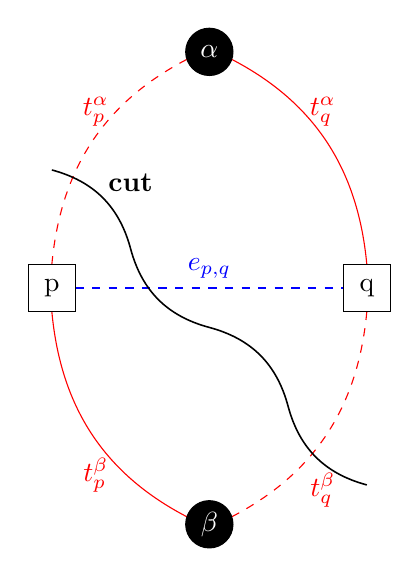
\begin{tikzpicture}
        \def\radi{0.3}
        \def\squ{0.3}
        \def\sqpos{2}

        
        
        %n-link
        \draw[dashed, line width=0.02cm, color=blue] (-\sqpos+\squ,0) -- node [midway, above] {$e_{p,q}$} (\sqpos-\squ,0);
      

        %t-link of p
        \draw[dashed,color=red](-\sqpos,0+\squ) to [bend left]node[midway, above] {$t_p^\alpha$}  (-0.3*\radi,3);
        \draw[color=red](-\sqpos,0-\squ) to [bend right]node[midway, below=0.1cm] {$t_p^\beta$} (-0.3*\radi,-3);
        
        %t-link of q
        \draw[color=red](+\sqpos,0+\squ) to [bend right]node[midway, above] {$t_q^\alpha$} (.3*\radi,3) ;
        \draw[dashed, color=red](+\sqpos,0-\squ) to [bend left]node[midway, below=0.3cm] {$t_q^\beta$}  (.3*\radi,-3);
        
        %cut
        \draw[line width =0.02cm] (-2,1.5) to [bend left]  (-1,0.5) node[above=0.6cm] {\textbf{cut} }to [bend right] (0,-0.5) to [bend left] (1,-1.5) to [bend right] (2,-2.5);


        %labels 
        \draw[fill=black] (0,-3) circle (\radi) node {\textcolor{white}{$\beta$}}; 
        \draw[fill=black] (0,3) circle (\radi) node {\textcolor{white}{$\alpha$}};
        %pixels 
        \draw[color=black] (-\sqpos-\squ,0-\squ) rectangle node{p} (-\sqpos+\squ,0+\squ);
        \draw[fill=white] (\sqpos-\squ,0-\squ) rectangle node{q} (\sqpos+\squ,0+\squ);

        
    \end{tikzpicture}
\end{document}
